\documentclass[tikz,border=10pt]{standalone}
\usepackage[T1]{fontenc}
\usepackage{lmodern}
\usepackage{xcolor}
\usetikzlibrary{arrows.meta,positioning,fit,calc,backgrounds,shadows}

\definecolor{ink}{HTML}{172033}
\definecolor{muted}{HTML}{536071}
\definecolor{blue}{HTML}{2F7DF6}
\definecolor{cyan}{HTML}{00A6D6}
\definecolor{green}{HTML}{18A957}
\definecolor{yellow}{HTML}{F7B731}
\definecolor{orange}{HTML}{F06A2F}
\definecolor{pink}{HTML}{DF4E9A}
\definecolor{violet}{HTML}{6F5BD6}
\definecolor{line}{HTML}{9AA8B8}

\tikzset{
  font=\sffamily,
  title/.style={
    font=\sffamily\bfseries\LARGE,
    text=ink,
    align=center
  },
  subtitle/.style={
    font=\sffamily\small,
    text=muted,
    align=center
  },
  lane/.style={
    draw=#1!55!black,
    fill=#1!4,
    very thick,
    rounded corners=8pt,
    inner sep=10pt
  },
  laneLabel/.style={
    font=\sffamily\bfseries\small,
    text=#1!55!black,
    align=left
  },
  phase/.style={
    draw=#1!70!black,
    fill=#1!10,
    very thick,
    rounded corners=5pt,
    minimum width=3.45cm,
    minimum height=1.35cm,
    align=center,
    text=ink,
    drop shadow={shadow xshift=.8pt,shadow yshift=-.8pt,opacity=.12}
  },
  facet/.style={
    draw=#1!58!black,
    fill=#1!7,
    thick,
    rounded corners=5pt,
    text width=4.35cm,
    minimum height=2.05cm,
    align=left,
    inner sep=8pt,
    text=ink
  },
  contract/.style={
    draw=#1!58!black,
    fill=#1!8,
    thick,
    rounded corners=5pt,
    text width=3.65cm,
    minimum height=1.55cm,
    align=left,
    inner sep=7pt,
    text=ink
  },
  agent/.style={
    draw=#1!68!black,
    fill=#1!12,
    thick,
    rounded corners=12pt,
    text width=4.35cm,
    minimum height=1.75cm,
    align=center,
    inner sep=8pt,
    text=ink
  },
  note/.style={
    draw=blue!55!black,
    fill=blue!4,
    thick,
    rounded corners=6pt,
    text width=24.4cm,
    align=left,
    inner sep=9pt,
    text=ink,
    font=\sffamily\scriptsize
  },
  arrow/.style={
    -{Latex[length=3.1mm,width=2mm]},
    very thick,
    draw=line
  },
  downarrow/.style={
    -{Latex[length=2.7mm,width=1.8mm]},
    thick,
    draw=line
  },
  small/.style={font=\sffamily\scriptsize, text=muted, align=center}
}

\begin{document}
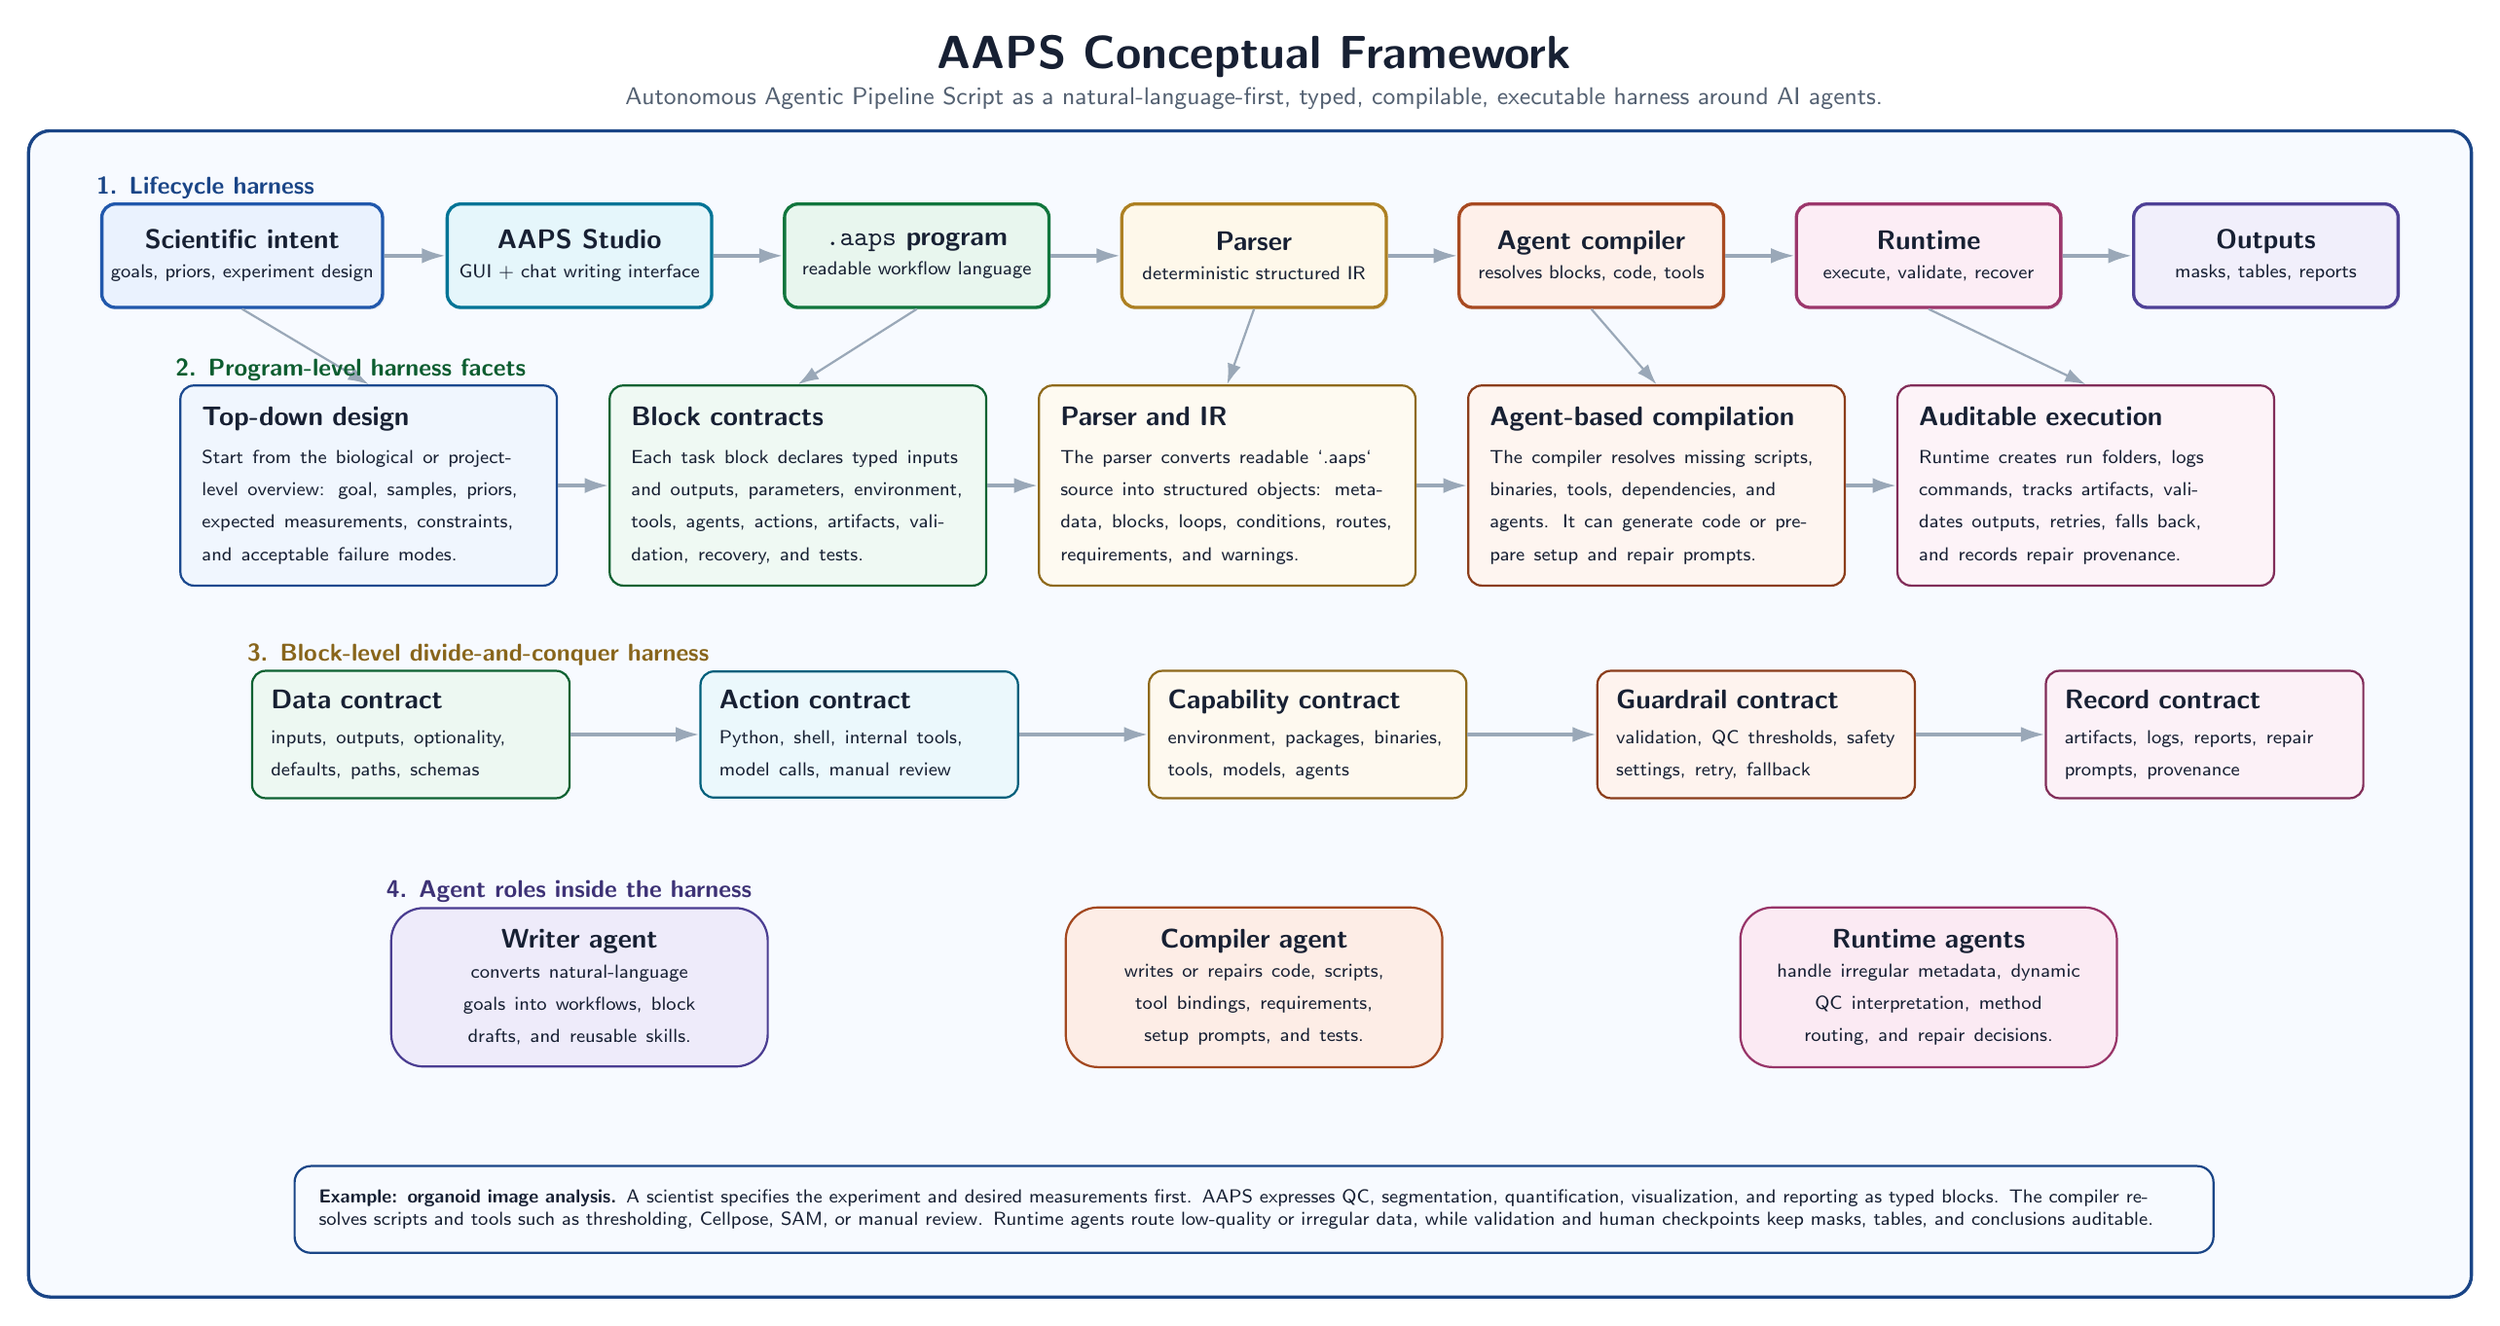
\begin{tikzpicture}[x=1cm,y=1cm]
  \node[title] at (13.2,15.7) {AAPS Conceptual Framework};
  \node[subtitle, text width=25cm] at (13.2,15.15)
    {Autonomous Agentic Pipeline Script as a natural-language-first, typed, compilable, executable harness around AI agents.};

  % Lane 1: lifecycle.
  \node[phase=blue]   (intent)   at (0,13.1) {\textbf{Scientific intent}\\[-1pt]\scriptsize goals, priors, experiment design};
  \node[phase=cyan]   (studio)   at (4.4,13.1) {\textbf{AAPS Studio}\\[-1pt]\scriptsize GUI + chat writing interface};
  \node[phase=green]  (script)   at (8.8,13.1) {\textbf{\texttt{.aaps} program}\\[-1pt]\scriptsize readable workflow language};
  \node[phase=yellow] (parser)   at (13.2,13.1) {\textbf{Parser}\\[-1pt]\scriptsize deterministic structured IR};
  \node[phase=orange] (compiler) at (17.6,13.1) {\textbf{Agent compiler}\\[-1pt]\scriptsize resolves blocks, code, tools};
  \node[phase=pink]   (runtime)  at (22,13.1) {\textbf{Runtime}\\[-1pt]\scriptsize execute, validate, recover};
  \node[phase=violet] (outputs)  at (26.4,13.1) {\textbf{Outputs}\\[-1pt]\scriptsize masks, tables, reports};

  \foreach \a/\b in {intent/studio,studio/script,script/parser,parser/compiler,compiler/runtime,runtime/outputs}
    \draw[arrow] (\a) -- (\b);

  \begin{scope}[on background layer]
    \node[lane=blue, fit=(intent)(studio)(script)(parser)(compiler)(runtime)(outputs)] (lifecycleLane) {};
  \end{scope}
  \node[laneLabel=blue, anchor=west] at ($(lifecycleLane.north west)+(0.2,-0.18)$) {1. Lifecycle harness};

  % Lane 2: harness facets.
  \node[facet=blue] (design) at (1.65,10.1) {
    \textbf{Top-down design}\\[2pt]
    \scriptsize
    Start from the biological or project-level overview: goal, samples,
    priors, expected measurements, constraints, and acceptable failure modes.
  };
  \node[facet=green] (contracts) at (7.25,10.1) {
    \textbf{Block contracts}\\[2pt]
    \scriptsize
    Each task block declares typed inputs and outputs, parameters, environment,
    tools, agents, actions, artifacts, validation, recovery, and tests.
  };
  \node[facet=yellow] (ir) at (12.85,10.1) {
    \textbf{Parser and IR}\\[2pt]
    \scriptsize
    The parser converts readable `.aaps` source into structured objects:
    metadata, blocks, loops, conditions, routes, requirements, and warnings.
  };
  \node[facet=orange] (compile) at (18.45,10.1) {
    \textbf{Agent-based compilation}\\[2pt]
    \scriptsize
    The compiler resolves missing scripts, binaries, tools, dependencies, and
    agents. It can generate code or prepare setup and repair prompts.
  };
  \node[facet=pink] (execution) at (24.05,10.1) {
    \textbf{Auditable execution}\\[2pt]
    \scriptsize
    Runtime creates run folders, logs commands, tracks artifacts, validates
    outputs, retries, falls back, and records repair provenance.
  };

  \foreach \a/\b in {design/contracts,contracts/ir,ir/compile,compile/execution}
    \draw[arrow] (\a) -- (\b);

  \draw[downarrow] (intent.south) -- (design.north);
  \draw[downarrow] (script.south) -- (contracts.north);
  \draw[downarrow] (parser.south) -- (ir.north);
  \draw[downarrow] (compiler.south) -- (compile.north);
  \draw[downarrow] (runtime.south) -- (execution.north);

  \begin{scope}[on background layer]
    \node[lane=green, fit=(design)(contracts)(ir)(compile)(execution)] (facetLane) {};
  \end{scope}
  \node[laneLabel=green, anchor=west] at ($(facetLane.north west)+(0.2,-0.18)$) {2. Program-level harness facets};

  % Lane 3: block contract decomposition.
  \node[contract=green] (data) at (2.2,6.85) {
    \textbf{Data contract}\\[1pt]
    \scriptsize inputs, outputs, optionality, defaults, paths, schemas
  };
  \node[contract=cyan] (actions) at (8.05,6.85) {
    \textbf{Action contract}\\[1pt]
    \scriptsize Python, shell, internal tools, model calls, manual review
  };
  \node[contract=yellow] (capability) at (13.9,6.85) {
    \textbf{Capability contract}\\[1pt]
    \scriptsize environment, packages, binaries, tools, models, agents
  };
  \node[contract=orange] (guardrails) at (19.75,6.85) {
    \textbf{Guardrail contract}\\[1pt]
    \scriptsize validation, QC thresholds, safety settings, retry, fallback
  };
  \node[contract=pink] (records) at (25.6,6.85) {
    \textbf{Record contract}\\[1pt]
    \scriptsize artifacts, logs, reports, repair prompts, provenance
  };

  \foreach \a/\b in {data/actions,actions/capability,capability/guardrails,guardrails/records}
    \draw[arrow] (\a) -- (\b);

  \begin{scope}[on background layer]
    \node[lane=yellow, fit=(data)(actions)(capability)(guardrails)(records)] (blockLane) {};
  \end{scope}
  \node[laneLabel=yellow, anchor=west] at ($(blockLane.north west)+(0.2,-0.18)$) {3. Block-level divide-and-conquer harness};

  % Lane 4: agent roles.
  \node[agent=violet] (writer) at (4.4,3.55) {
    \textbf{Writer agent}\\[-1pt]
    \scriptsize converts natural-language goals into workflows, block drafts,
    and reusable skills.
  };
  \node[agent=orange] (compileragent) at (13.2,3.55) {
    \textbf{Compiler agent}\\[-1pt]
    \scriptsize writes or repairs code, scripts, tool bindings, requirements,
    setup prompts, and tests.
  };
  \node[agent=pink] (runtimeagent) at (22,3.55) {
    \textbf{Runtime agents}\\[-1pt]
    \scriptsize handle irregular metadata, dynamic QC interpretation, method
    routing, and repair decisions.
  };

  \begin{scope}[on background layer]
    \node[lane=violet, fit=(writer)(compileragent)(runtimeagent)] (agentLane) {};
  \end{scope}
  \node[laneLabel=violet, anchor=west] at ($(agentLane.north west)+(0.2,-0.18)$) {4. Agent roles inside the harness};

  % Example strip.
  \node[note] (example) at (13.2,0.65) {
    \textbf{Example: organoid image analysis.}
    A scientist specifies the experiment and desired measurements first. AAPS
    expresses QC, segmentation, quantification, visualization, and reporting as
    typed blocks. The compiler resolves scripts and tools such as thresholding,
    Cellpose, SAM, or manual review. Runtime agents route low-quality or
    irregular data, while validation and human checkpoints keep masks, tables,
    and conclusions auditable.
  };

  \begin{scope}[on background layer]
    \node[lane=blue, fit=(lifecycleLane)(facetLane)(blockLane)(agentLane)(example),
      inner sep=16pt] {};
  \end{scope}
\end{tikzpicture}
\end{document}
